\section{Method}
\label{sec:method}

\subsection{Method Overview}
\label{sec:method_overview}

MapPolicy is a structured imitation learning framework that incorporates an explicit Scene Map.
At each time step, the system first constructs a scene graph from the current RGB-D observation, then encodes the graph into compact map features, and finally fuses these features with visual evidence and robot state for action prediction. In compact form, $\mathcal{G}_t = F_{\mathrm{ctor}}(I_t, D_t)$, $\mathbf{z}_{map} = F_{\mathrm{enc}}(\mathcal{G}_t)$, and $\hat{a}_t = \pi_\theta(\mathbf{z}_{map}, \mathbf{z}_{vis}, \mathbf{z}_{state})$, where $I_t$ and $D_t$ denote RGB and depth observations, $\mathbf{z}_{vis}=F_{\mathrm{vis}}(I_t)$ is the visual feature, and $\mathbf{z}_{state}=F_{\mathrm{state}}(s_t)$ is the robot state feature.

Figure~\ref{fig:pipeline} summarizes the full pipeline.
\textit{Map Constructor} instantiates Scene Map from sensor observations, \textit{Map Encoder} turns the graph into relation-aware map features, and the \textit{Policy Backbone} combines these features with visual and proprioceptive features to predict actions.
This decomposition makes the role of Scene Map explicit: it is not an external annotation consumed only during training, but the intermediate representation through which the policy reasons about scene organization under partial observability.

\begin{figure}[t]
    \centering
    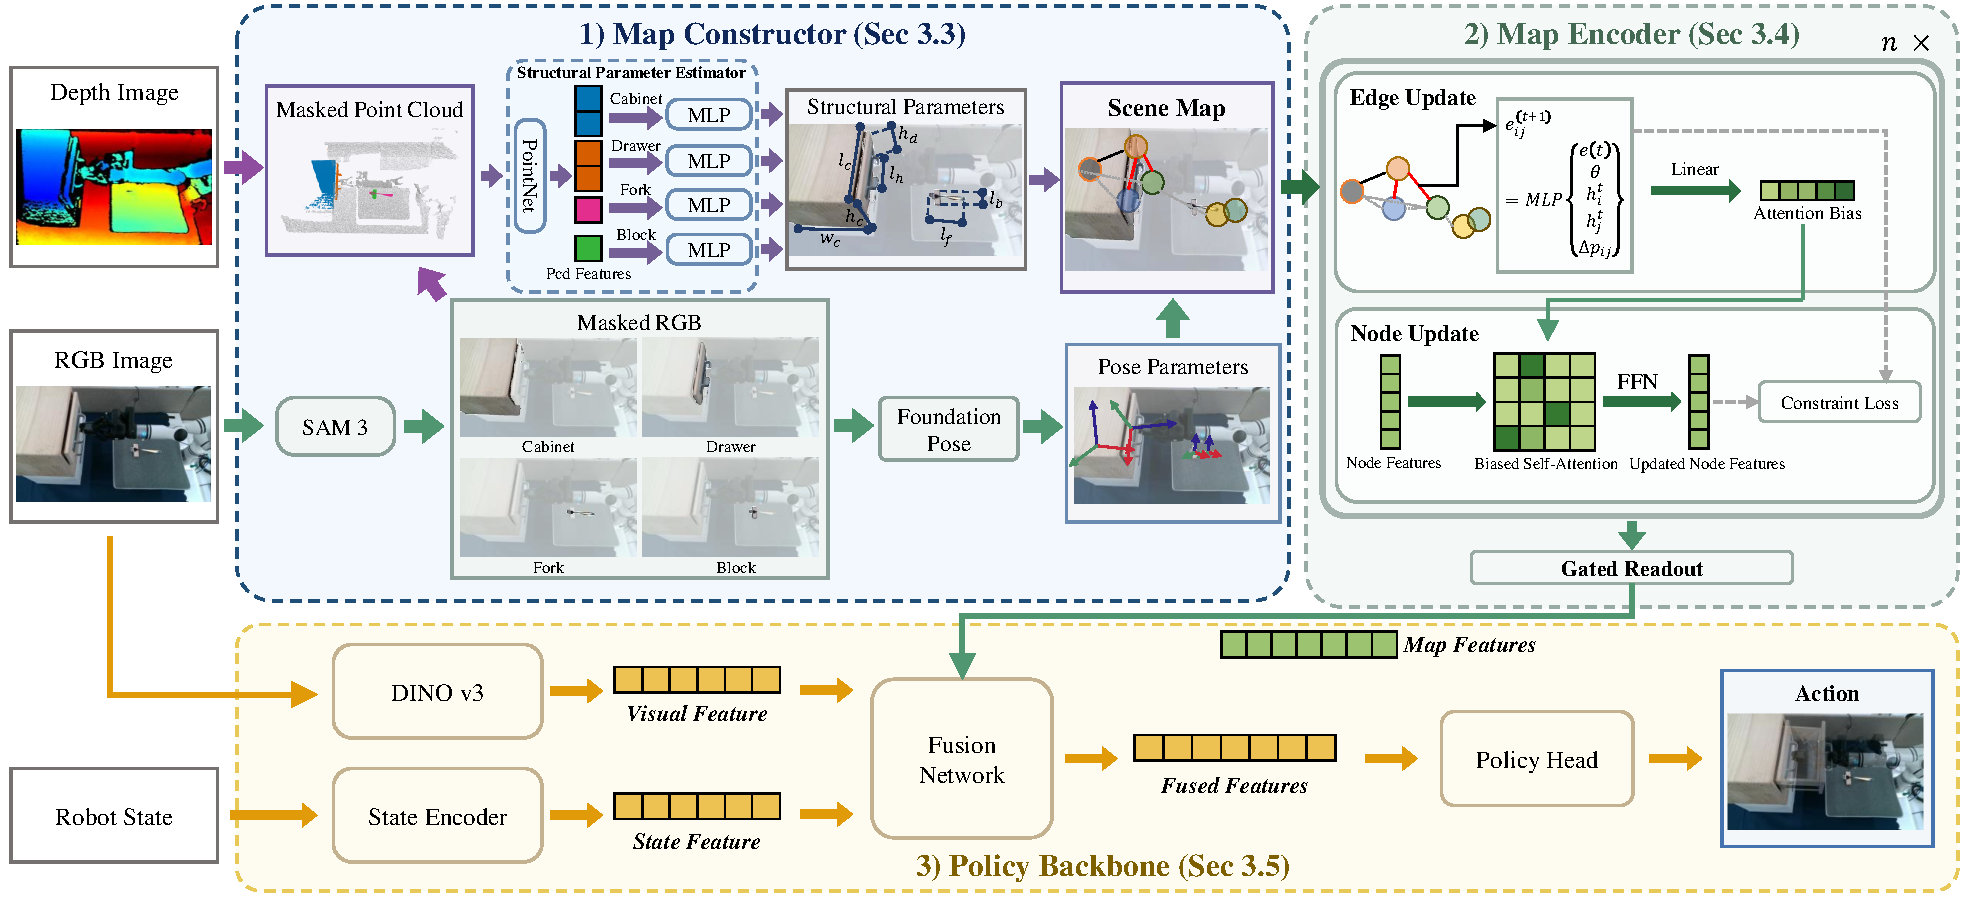
\includegraphics[width=0.95\linewidth]{figs/Pipeline.pdf}
    \caption{Overall pipeline of MapPolicy. The Map Constructor instantiates a Scene Map from RGB-D observations, the Map Encoder transforms the graph into map features, and the Policy Backbone fuses these features with visual and robot state information for action prediction.}
    \label{fig:pipeline}
\end{figure}

\subsection{Scene Map}
\label{sec:method_scene_map}

As shown in fig.~\ref{fig:scenemap}, Scene Map is a structured representation. It represents a manipulation scene as a graph $\mathcal{G}=(\mathcal{V},\mathcal{E})$. Each object is represented as an object-level subgraph, and the full scene map is obtained by composing these subgraphs together with cross-object relations. In the Scene Map example in fig.~\ref{fig:scenemap}, object parts are decomposed into primitives, and their connectivity forms a graph that preserves object structure and spatial layout even when some parts are not directly visible.

The nodes in Scene Map correspond to geometric primitives, including cuboids, cylinders, spheres, and rings as illustrated in fig.~\ref{fig:scenemap}. A node stores the primitive pose, shape or scale parameters, semantic identity, and affordance-related geometry. In compact form, we write a node as $v_i=\langle \mathbf{p}_i,\mathbf{r}_i,X_i^{pos},s_i,X_i^{aff}\rangle$, where $X_i^{pos}$ samples the primitive geometry and $X_i^{aff}$ samples manipulation-relevant regions. This primitive-level decomposition preserves object shape and part layout without collapsing them into a single object descriptor.

The edges in Scene Map represent physical constraints between primitives. Each edge is written as $e_{ij}=\langle c_{ij},\theta_{ij},a_{ij},T_{ij}\rangle$, where $c_{ij}$ is the constraint type, $\theta_{ij}$ contains continuous relation parameters, $a_{ij}$ selects the geometric anchors used by the relation, and $T_{ij}$ is the relative pose. These constraints are derived from the local geometry of primitives. For example, face anchors provide contact planes and normal directions, while axis anchors provide center lines and axial directions. The right part of fig.~\ref{fig:scenemap} describes the allowed motion of primitive B relative to primitive A, where red crosses denote forbidden translation or rotation and green arrows denote free degrees of freedom. For example, a cylindrical constraint is defined between two axis anchors: it enforces the two axes to be coaxial by constraining their direction mismatch and radial offset, while leaving translation along the axis and rotation around the axis unconstrained. Detailed primitive definitions and all six constraint types are provided in Appendix~\ref{app:scene_map_constraint}.

\begin{figure}[t]
    \centering
    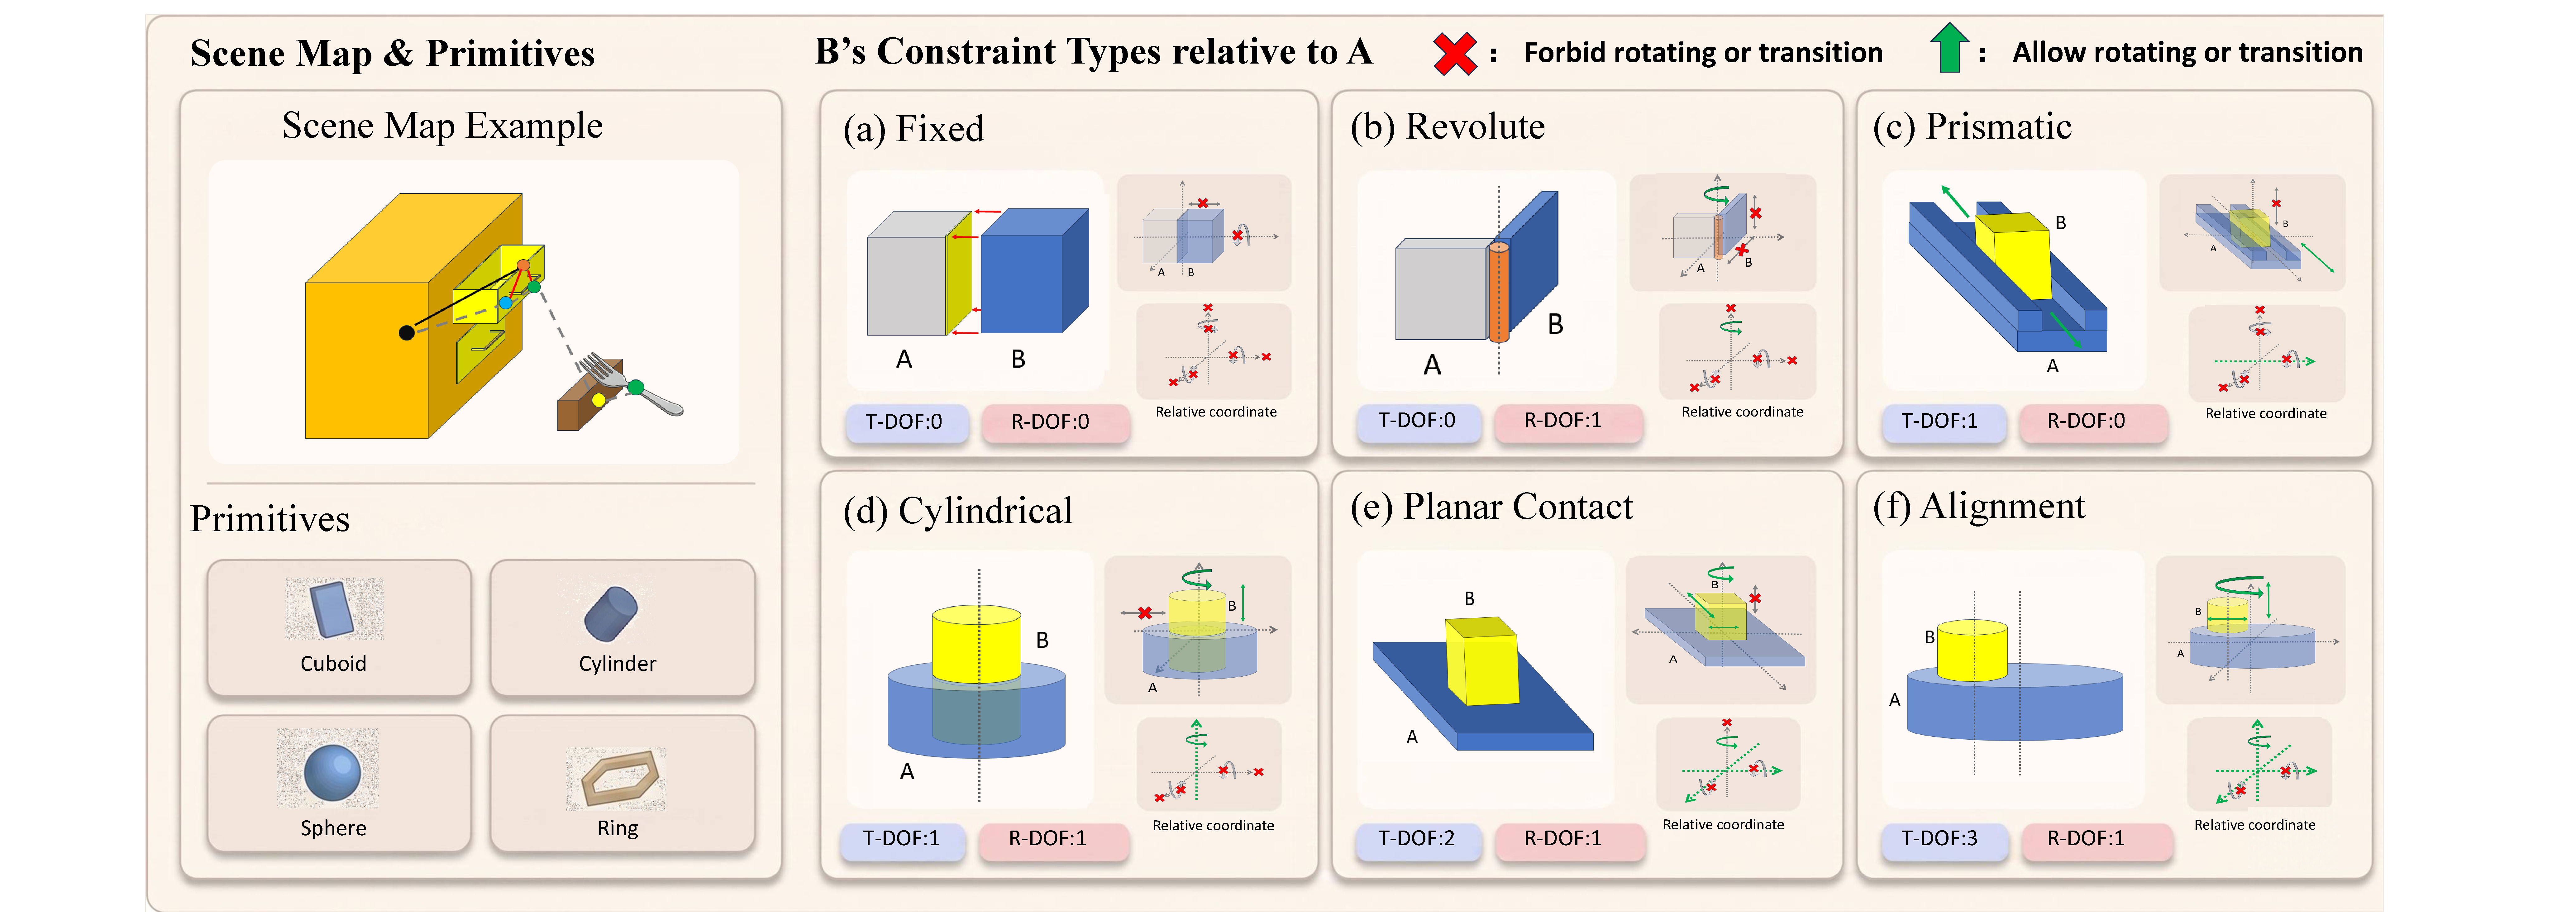
\includegraphics[width=0.95\linewidth]{figs/scenemap.pdf}
    \caption{Scene Map. The left panel shows a scene-map example and the primitive set used to decompose object structure, including cuboid, cylinder, sphere, and ring. The right panel summarizes the motion of object B relative to object A under six physical constraint types, where red crosses indicate forbidden translation or rotation and green arrows indicate allowed degrees of freedom.}
    \label{fig:scenemap}
\end{figure}

\subsection{Map Constructor}
\label{sec:map_constructor}

% As shown in fig.~\ref{fig:pipeline}(1), Map Constructor is the first module in the pipeline. Its role is to convert the current observation into an instantiated Scene Map, $\mathcal{G}_t = F_{\mathrm{ctor}}(I_t, D_t)$.

Scene Map defines \emph{what} structural information should be represented, while the constructor defines \emph{how} that information is instantiated from the current scene. Following the pipeline in fig.~\ref{fig:pipeline}, the observation is first organized into object-level evidence, including object geometry and pose estimates.

Firstly, SAM 3~\cite{sam3} is used to segment foreground objects from the RGB image, and FoundationPose~\cite{foundationposewen2024, bundlesdfwen2023} is then applied to estimate their pose parameters. In parallel, the depth image and object masks are projected into masked point clouds. A structural parameter estimator, implemented with PointNet~\cite{Qi2017PointNet} followed by separate MLP heads, encodes these point clouds and predicts the structural parameters. Finally, the estimated pose and structural parameters are combined to instantiate the Scene Map.


\subsection{Map Encoder}
\label{sec:map_encoder}

As shown in fig.~\ref{fig:pipeline}(2), Map Encoder transforms the instantiated Scene Map into compact map features $\mathbf{z}_{map} = F_{\mathrm{enc}}(\mathcal{G}_t)$ for control.
The encoder keeps node and edge streams separate at the input stage. For each node, primitive geometry, affordance samples, and semantic descriptors are embedded separately and fused into the initial node embedding $\mathbf{h}_i^0$. For each edge, relation type, continuous relation parameters, anchor descriptors, and relative pose are embedded and fused into the initial relation embedding $\mathbf{e}_{ij}^0$. This preserves both part-level attributes and explicit relation attributes before message passing.

For batched graph attention, the sparse Scene Map is packed into fixed-size node and edge tensors, $\mathbf{H}^0 \in \mathbb{R}^{B \times N \times d}$ and $\mathbf{E}^0 \in \mathbb{R}^{B \times N \times N \times d}$, where valid edge entries carry the relation attributes recovered by the constructor.
We apply a stack of Graphormer-style layers on these tensors, adapted from graph transformer mechanisms~\cite{Surveygraphtransformer, graphormer, rampasek2022GPS}. In each layer, each relation embedding is updated from its previous state and the two endpoint node states. The updated relation is then projected into a head-specific additive attention bias, which modulates node self-attention:
\begin{equation}
b_{ij,r}^{\ell} = \mathbf{w}_{b,r}^\top \mathbf{e}_{ij}^{\ell}, \qquad
\alpha_{ij,r}^{\ell} = \operatorname{softmax}_j\!\left(
\frac{(\mathbf{q}_{i,r}^{\ell})^\top \mathbf{k}_{j,r}^{\ell}}{\sqrt{d_h}} + b_{ij,r}^{\ell}
\right),
\end{equation}
where $r$ indexes attention heads. Node features are updated by the biased multi-head attention block followed by a feed-forward block with residual connections. Consequently, information can propagate between parts according to both node content and the explicit relation connecting them.
After the final layer, a gated readout computes attention weights over node states and sums them into $\mathbf{z}_{map}$. The resulting map feature is compact enough to fuse with visual and robot state features, while still being produced through edge-conditioned reasoning over the explicit Scene Map structure.

\subsection{Policy Backbone}
\label{sec:policy_backbone}

As shown in fig.~\ref{fig:pipeline}(3), Policy Backbone predicts actions from the fused multimodal representation. In parallel with map encoding, a visual encoder extracts $\mathbf{z}_{vis}$ from the current RGB observation, and a state encoder extracts $\mathbf{z}_{state}$ from proprioceptive input. The map feature, visual feature, and robot state feature are separately projected into modality tokens, fused by self-attention, and passed to an MLP policy head to predict $\hat{a}_t$.
The three branches play complementary roles. The visual branch captures currently visible evidence, the map branch provides structural priors and relation-aware context, and the state branch provides the robot's internal configuration. The policy backbone does not reconstruct scene structure again. It consumes the map features produced by the Map Encoder and turns the fused representation into a manipulation action.

\subsection{Loss Functions and Implementation Details}
\label{sec:loss_functions}
\label{sec:implementation_details}

MapPolicy uses losses at both stages of training. For Map Constructor training, the objective is $\mathcal{L}_{ctor}=\mathcal{L}_{pcd}+\lambda_{struct}\mathcal{L}_{struct}$. Here $\mathcal{L}_{pcd}$ compares the point cloud rendered from the predicted Scene Map and projected into the camera frame with the observed masked point cloud, while $\mathcal{L}_{struct}$ is a mean-squared error on structural parameters. This supervision encourages the constructed Scene Map to be both geometrically consistent with RGB-D observations and structurally aligned with the task-specific map template.

For policy training, the objective is $\mathcal{L}_{policy}=\mathcal{L}_{act}+\lambda_{phys}\mathcal{L}_{phys}$. The action loss $\mathcal{L}_{act}$ is the imitation loss on expert actions. The physical constraint loss $\mathcal{L}_{phys}$ regularizes map features by decoding edge-conditioned representations into anchor states and penalizing violations of the corresponding geometric or kinematic constraints. Detailed constraint residuals are provided in Appendix~\ref{app:scene_map_constraint}.

MapPolicy is trained in two stages. We first train the structural parameter estimator in the Map Constructor, and then freeze the constructor while training the Map Encoder and Policy Backbone. At inference time, the system follows the same observation-to-map-to-action pipeline: RGB-D observations provide object masks, poses, and masked point clouds, which instantiate a Scene Map that is encoded and fused with visual and robot state features for action prediction. The policy backbone uses a linear state encoder, attention-based multimodal fusion, and an MLP policy head. Full implementation details are provided in Appendix~\ref{app:implementation_details}.
